\chapter{Sample a Test Set} \label{chapter:sample_test_set}
The test set will be used to evaluate performance of a very final model
and forecast the score in the competitions leaderboard. It may seems like
it's to early to create a test set, but I'll do it to prevent data snooping.

I'm going to do stratified sampling with scikit-learn's StraifiedShuffleSplit
to maintain equal ratio of men and women in the train set and the test set.
Women seem to have had a better chance of surviving due to the "women and
children first" protocol for loading lifeboats.

First, let's check how many passengers survived. Figure 
\ref{number_of_survivors} illustrates these numbers. There are 342 (38.38\%)
survived passengers and 549 (61.62\%) drowned passengers in the dataset, 
so the dataset is a bit skewed. However, it's most likely, there will be 
enough representatives of both classes in the test set.

\begin{figure}[!ht]
	\centering
	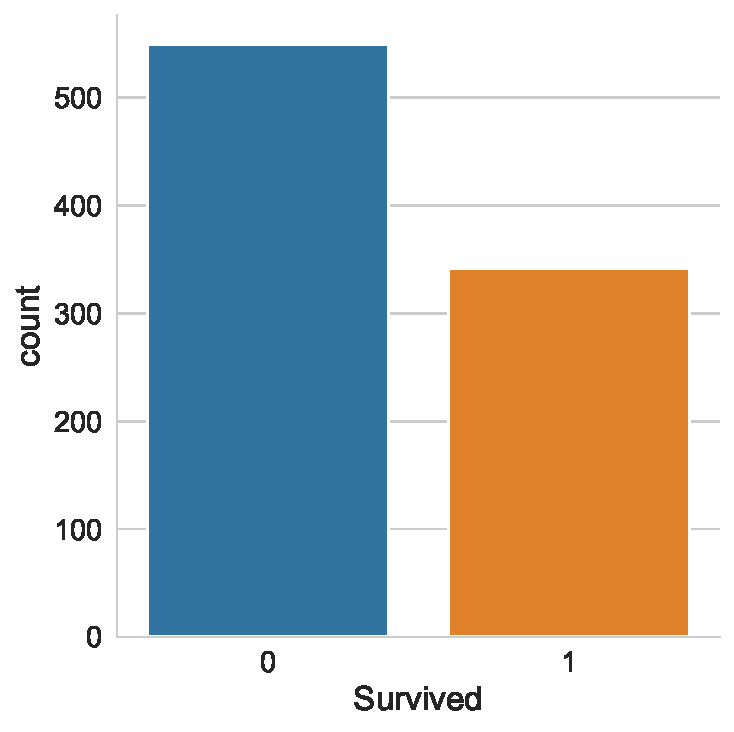
\includegraphics[width=0.5\textwidth]{number_of_survivors}
	\caption{Number of survived and drowned passangers in whole dataset}
	\label{number_of_survivors}
\end{figure}

Next, let's check the proportion of women among all survivors (figure
\ref{proportion_of_survived_women}), and check the proportion of survived
women in each \textbf{"Pclass"} (figure 
\ref{proportion_of_survived_women_among_pclasses}).

\begin{figure}[!ht]
	\centering
	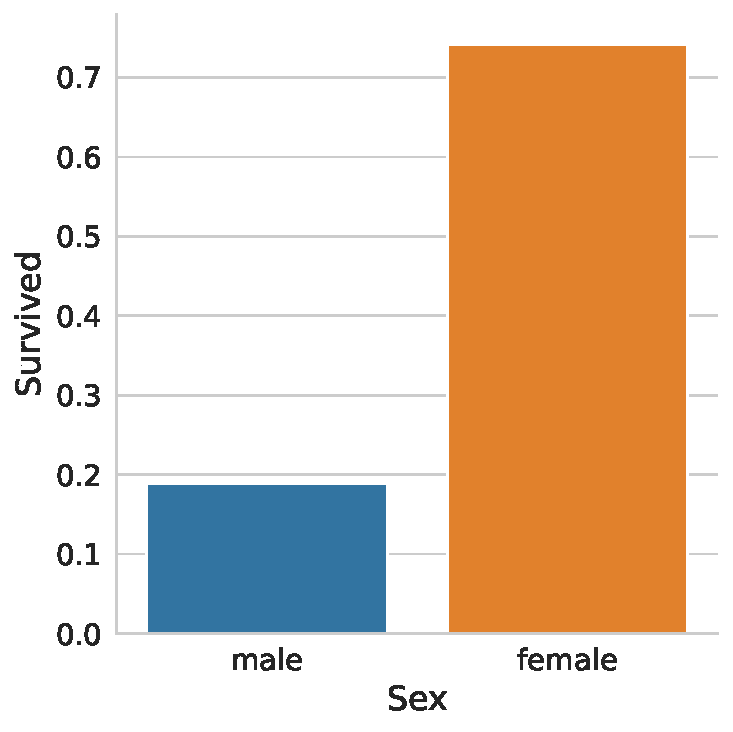
\includegraphics[width=0.5\textwidth]{proportion_of_survived_women}
	\caption{Proportions of survived men and women}
	\label{proportion_of_survived_women}
\end{figure}

\begin{figure}[!ht]
	\centering
	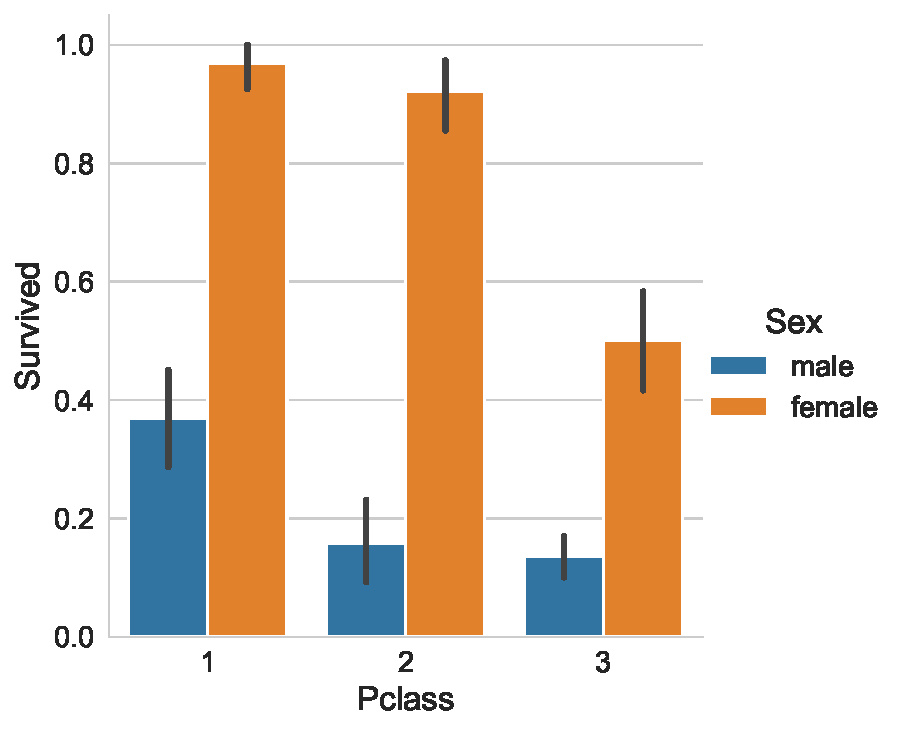
\includegraphics[width=0.5\textwidth]{proportion_of_survived_women_among_pclasses}
	\caption{Proporotion of survived women and men in each \textbf{"Pclass"}}
	\label{proportion_of_survived_women_among_pclasses}
\end{figure}

Figures \ref{proportion_of_survived_women} and 
\ref{proportion_of_survived_women_among_pclasses} show that in the entire 
dataset and in each \textbf{"Pclass"}, there are more female survivors 
than males. Thus it is reasonable to do stratification based on the
passenger's gender. I will use 80\% of the data for training and hold 
out 20\% for testing, refer to the Jupyter Notebook for details.